% !TeX document-id = {f19fb972-db1f-447e-9d78-531139c30778}
% !BIB program = biber

%\documentclass[handout]{beamer}
\documentclass[compress]{beamer}
\usepackage[T1]{fontenc}
\usetheme[block=fill,subsectionpage=progressbar,sectionpage=progressbar]{metropolis} 
\usepackage{graphicx}

\usepackage{wasysym}
\usepackage{etoolbox}
\usepackage[utf8]{inputenc}

\usepackage{pifont}

\usepackage{threeparttable}
\usepackage{subcaption}

\usepackage{tikz-qtree}
\setbeamercovered{still covered={\opaqueness<1->{5}},again covered={\opaqueness<1->{100}}}


\usepackage{listings}

\lstset{
	basicstyle=\scriptsize\ttfamily,
	columns=flexible,
	breaklines=true,
	numbers=left,
	%stepsize=1,
	numberstyle=\tiny,
	backgroundcolor=\color[rgb]{0.85,0.90,1}
}



\lstnewenvironment{lstlistingoutput}{\lstset{basicstyle=\footnotesize\ttfamily,
		columns=flexible,
		breaklines=true,
		numbers=left,
		%stepsize=1,
		numberstyle=\tiny,
		backgroundcolor=\color[rgb]{.7,.7,.7}}}{}


\lstnewenvironment{lstlistingoutputtiny}{\lstset{basicstyle=\tiny\ttfamily,
		columns=flexible,
		breaklines=true,
		numbers=left,
		%stepsize=1,
		numberstyle=\tiny,
		backgroundcolor=\color[rgb]{.7,.7,.7}}}{}


\usepackage[american]{babel}
\usepackage{csquotes}
\usepackage[style=apa, backend = biber]{biblatex}
\DeclareLanguageMapping{american}{american-UoN}
\addbibresource{../../literature.bib}
\renewcommand*{\bibfont}{\tiny}

\usepackage{tikz}
\usetikzlibrary{shapes,arrows,matrix}
\usepackage{multicol}

\usepackage{subcaption}

\usepackage{booktabs}
\usepackage{graphicx}



\makeatletter
\setbeamertemplate{headline}{%
	\begin{beamercolorbox}[colsep=1.5pt]{upper separation line head}
	\end{beamercolorbox}
	\begin{beamercolorbox}{section in head/foot}
		\vskip2pt\insertnavigation{\paperwidth}\vskip2pt
	\end{beamercolorbox}%
	\begin{beamercolorbox}[colsep=1.5pt]{lower separation line head}
	\end{beamercolorbox}
}
\makeatother



\setbeamercolor{section in head/foot}{fg=normal text.bg, bg=structure.fg}



\newcommand{\question}[1]{
	\begin{frame}[plain]
	\begin{columns}
		\column{.3\textwidth}
		\makebox[\columnwidth]{
			
\includegraphics[width=\columnwidth,height=\paperheight,keepaspectratio]{../../pictures/mannetje.png}}
		\column{.7\textwidth}
		\large
		\textcolor{orange}{\textbf{\emph{#1}}}
	\end{columns}
\end{frame}}


\begin{document}

\title[Big Data and Automated Content Analysis]{\textbf{A Practical Introduction to Machine Learning in Python} \\Day 3 - Wednesday \\ »Unsupervised Machine Learning«}
\author[Damian Trilling, Anne Kroon]{Damian Trilling \\ Anne Kroon \\ ~ \\ \footnotesize{d.c.trilling@uva.nl, @damian0604 \\a.c.kroon@uva.nl, @annekroon} \\}
\date{September 27, 2023}
\institute[Gesis]{Gesis}


\tikzstyle{block} = [rectangle, draw, fill=blue!20, 
text width=5em, text centered, rounded corners, minimum height=4em]
\tikzstyle{line} = [draw]
\tikzstyle{pijltje} = [draw, -latex']
\tikzstyle{cloud} = [draw, ellipse,fill=red!20, node distance=3cm,
minimum height=2em, text width=4em, text centered,]



\setbeamercovered{transparent}

\begin{frame}{}
\titlepage
\end{frame}

\begin{frame}{Today}
\tableofcontents
\end{frame}




\section[Automated Content Analysis]{Types of Automated Content Analysis}
\begin{frame}{}
Recap: Types of Automated Content Analysis
\end{frame}
\subsection*{Top-down vs. bottom-up}


%{\setbeamercolor{background canvas}{bg=black}
\begin{frame}[plain]
\makebox[\linewidth]{
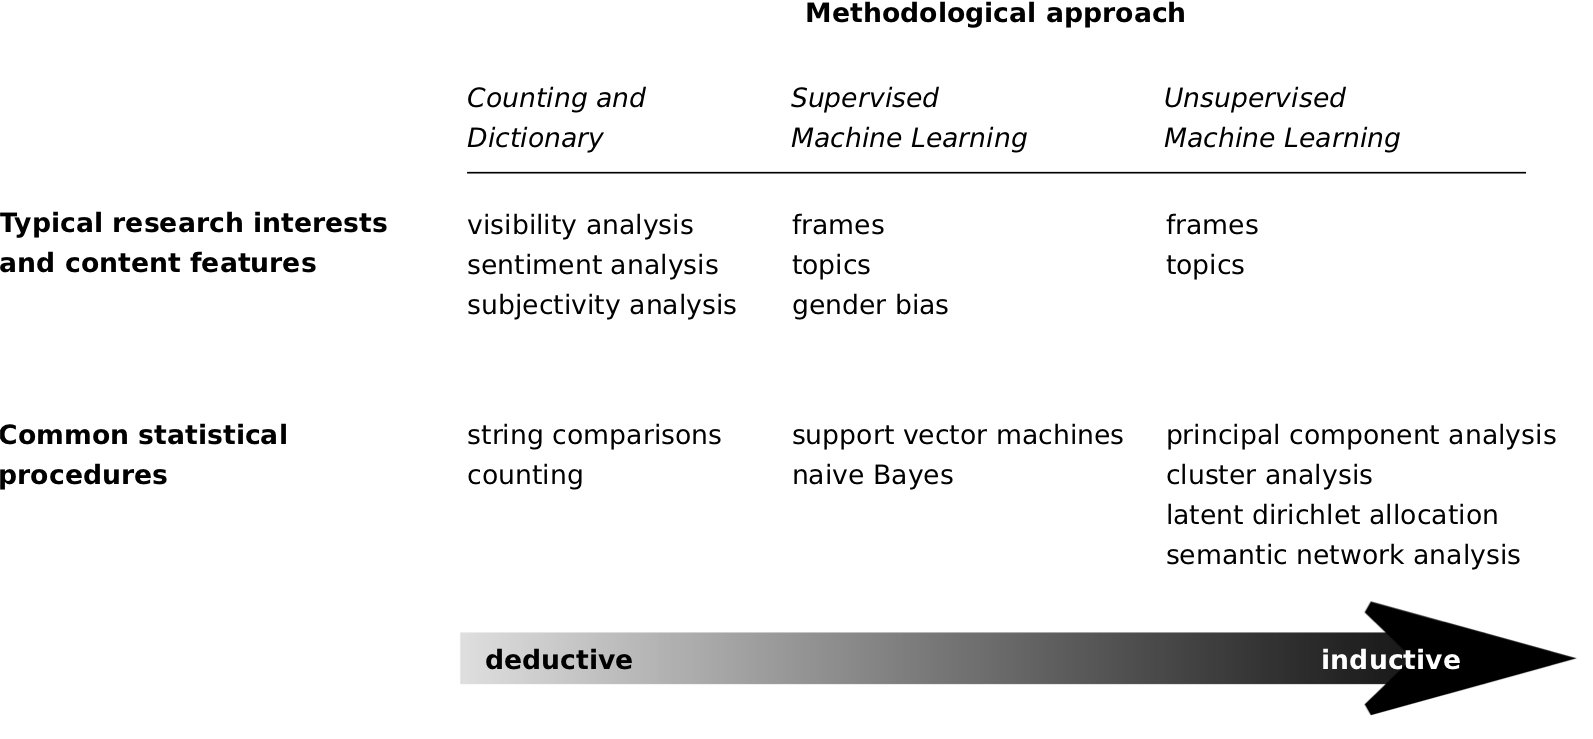
\includegraphics[width=\paperwidth,height=\paperheight,keepaspectratio]{../../pictures/boumanstrilling2016_}}
\end{frame}
%}




\begin{frame}[plain]
\makebox[\linewidth]{
	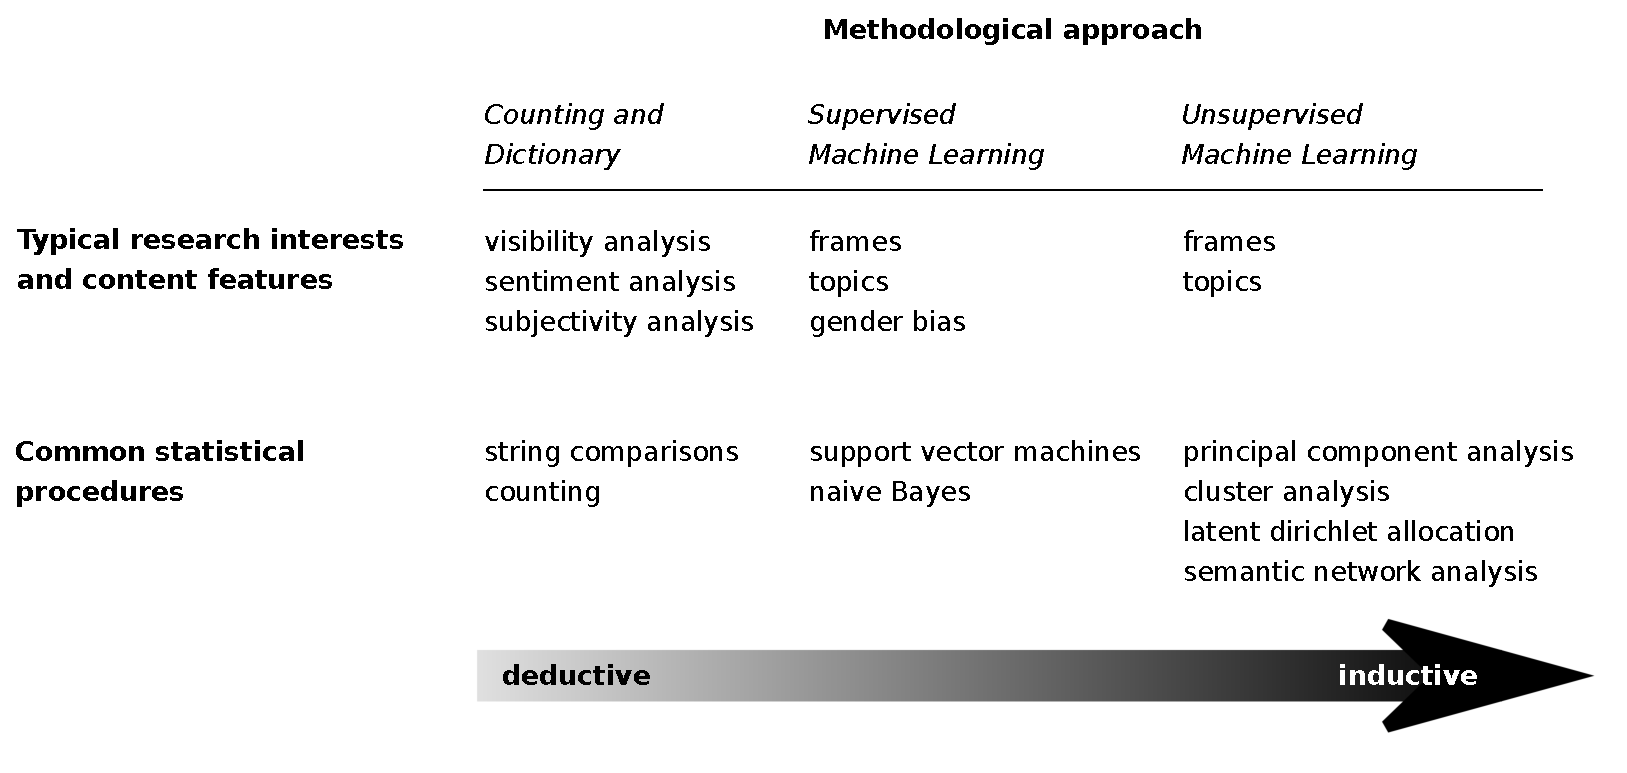
\includegraphics[width=\paperwidth,height=\paperheight,keepaspectratio]{../../pictures/boumanstrilling2016}}
\cite{Boumans2016}
\pause

\textbf{\textcolor{orange}{The same logic applies to non-textual data!}}
\end{frame}
%}




\begin{frame}{Some terminology }
\begin{columns}[t]
\column{.5\textwidth}

\begin{block}<1-4>{Supervised machine learning}
	You have a dataset with both predictor and outcome (independent and dependent variables; features and labels) --- a \emph{labeled} dataset.
	\onslide<2>{
		\footnotesize{Think of regression: You measured \texttt{x1}, \texttt{x2}, \texttt{x3} and you want to predict \texttt{y}, which you also measured}}
\end{block}

\column{.5\textwidth}

\begin{block}<3->{Unsupervised machine learning}
	You have no labels. \onslide<4>{(\footnotesize{You did not measure \texttt{y})}}\\
	\onslide<5>{\textbf{You might already be familiar with some techniques to figure out whether \texttt{x1}, \texttt{x2},\ldots \texttt{x\_i} co-occur} \begin{itemize}
			\item Principal Component Analysis (PCA) and Singular Value Decomposition (SVD)
			\item Cluster analysis
			\item Topic modelling (Non-negative matrix factorization and Latent Dirichlet Allocation)
			\item \ldots
		\end{itemize}
	}
\end{block}

\end{columns}

\end{frame}


\begin{frame}{Let's distinguish four use cases\ldots}

\begin{enumerate}
\item Finding similar variables (dimensionality reduction) -- unsupervised
\item Finding similar cases (clustering) -- unsupervised
\item Predicting a continous variable (regression) -- supervised
\item Predicting group membership (classification) -- supervised
\end{enumerate}
\end{frame}


\begin{frame}[plain]
\begin{table}[]
\resizebox{\textwidth}{!}{%
\begin{tabular}{lllllll}
& x1 & x2 & x3 & x4 & x5 & y \\
case1 & \ding{110}  & \ding{110}  & \ding{110}  & \ding{110}  & \ding{110} & \ding{110} \\
case2 & \ding{110}  & \ding{110}  & \ding{110}  & \ding{110}  & \ding{110} & \ding{110}\\
case3 & \ding{110}  & \ding{110}  & \ding{110}  & \ding{110}  & \ding{110} & \ding{110}\\
case4 & \ding{110}  & \ding{110}  & \ding{110}  & \ding{110}  & \ding{110} & \ding{110}\\
\end{tabular}%
}
\end{table}
\end{frame}



\begin{frame}[plain]
\begin{table}[]
\resizebox{\textwidth}{!}{%
\begin{tabular}{lllllll}
& \textcolor{orange}{x1} & x2 & \textcolor{orange}{x3}& \textcolor{blue}{x4} & \textcolor{blue}{x5} & \textcolor{gray}{(y)} \\
case1 & \textcolor{orange}{\ding{110}}  & \ding{110}  & \textcolor{orange}{\ding{110}}  & \textcolor{blue}{\ding{110}} & \textcolor{blue}{\ding{110}} & \textcolor{gray}{(\ding{110})} \\
case2 & \textcolor{orange}{\ding{110}}  & \ding{110}  & \textcolor{orange}{\ding{110}}  & \textcolor{blue}{\ding{110}} & \textcolor{blue}{\ding{110}} & \textcolor{gray}{(\ding{110})} \\
case3 & \textcolor{orange}{\ding{110}}  & \ding{110}  & \textcolor{orange}{\ding{110}}  & \textcolor{blue}{\ding{110}} & \textcolor{blue}{\ding{110}} & \textcolor{gray}{(\ding{110})} \\
case4 & \textcolor{orange}{\ding{110}}  & \ding{110}  & \textcolor{orange}{\ding{110}}  & \textcolor{blue}{\ding{110}} & \textcolor{blue}{\ding{110}} & \textcolor{gray}{(\ding{110})} \\
\end{tabular}%
}
\end{table}
Dimensionality reduction: finding similar variables (features)
\end{frame}


\begin{frame}[plain]
\begin{table}[]
\resizebox{\textwidth}{!}{%
\begin{tabular}{lllllll}
& x1 & x2 & x3 & x4 & x5 & \textcolor{gray}{(y)} \\
\textcolor{orange}{case1} & \textcolor{orange}{\ding{110}}  & \textcolor{orange}{\ding{110}}  &\textcolor{orange}{\ding{110}}  &\textcolor{orange}{\ding{110}}   & \textcolor{orange}{\ding{110}} & \textcolor{gray}{(\ding{110})} \\
\textcolor{blue}{case2} & \textcolor{blue}{\ding{110}}  & \textcolor{blue}{\ding{110}}  &\textcolor{blue}{\ding{110}}  &\textcolor{blue}{\ding{110}}   & \textcolor{blue}{\ding{110}} & \textcolor{gray}{(\ding{110})} \\
\textcolor{orange}{case3} & \textcolor{orange}{\ding{110}}  & \textcolor{orange}{\ding{110}}  &\textcolor{orange}{\ding{110}}  &\textcolor{orange}{\ding{110}}   & \textcolor{orange}{\ding{110}} & \textcolor{gray}{(\ding{110})} \\
\textcolor{orange}{case4} & \textcolor{orange}{\ding{110}}  & \textcolor{orange}{\ding{110}}  &\textcolor{orange}{\ding{110}}  &\textcolor{orange}{\ding{110}}   & \textcolor{orange}{\ding{110}} & \textcolor{gray}{(\ding{110})} \\
\end{tabular}%
}
\end{table}
Clustering: finding similar cases
\end{frame}



\begin{frame}[plain]
\begin{table}[]
\resizebox{\textwidth}{!}{%
\begin{tabular}{llllllll}
& x1 & x2 & x3 & x4 & x5 & $\rightarrow$ & \textcolor{orange}{y} \\
case1 & \ding{110}  & \ding{110}  & \ding{110}  & \ding{110}  & \ding{110} & $\rightarrow$ &\textcolor{orange}{\ding{110}}  \\
case2 & \ding{110}  & \ding{110}  & \ding{110}  & \ding{110}  & \ding{110} & $\rightarrow$ &\textcolor{orange}{\ding{110}} \\
case3 & \ding{110}  & \ding{110}  & \ding{110}  & \ding{110}  & \ding{110} & $\rightarrow$ &\textcolor{orange}{\ding{110}} \\
case4 & \ding{110}  & \ding{110}  & \ding{110}  & \ding{110}  & \ding{110} & $\rightarrow$ &\textcolor{orange}{\ding{110}} \\
&&&&&&& \\
new case & \ding{110}  & \ding{110}  & \ding{110}  & \ding{110}  & \ding{110} & $\rightarrow$ &\textbf{\textcolor{orange}{?}} \\
\end{tabular}%
}
Regression and classification: learn how to predict $y$.
\end{table}
\end{frame}




\begin{frame}[plain]
\textbf{Note, again, that the \ding{110} signs can be \emph{anything}}.
For us, often word counts or $tf\cdot$ idf scores ($x$) and, for supervised approaches, a topic, a sentiment, or similar ($y$). 

But it could also be pixel colors or clicks on links or anything else.
\begin{table}[]
\resizebox{\textwidth}{!}{%
\begin{tabular}{lllllll}
& x1 & x2 & x3 & x4 & x5 & y \\
case1 & \ding{110}  & \ding{110}  & \ding{110}  & \ding{110}  & \ding{110} & \ding{110} \\
case2 & \ding{110}  & \ding{110}  & \ding{110}  & \ding{110}  & \ding{110} & \ding{110}\\
case3 & \ding{110}  & \ding{110}  & \ding{110}  & \ding{110}  & \ding{110} & \ding{110}\\
case4 & \ding{110}  & \ding{110}  & \ding{110}  & \ding{110}  & \ding{110} & \ding{110}\\
\end{tabular}%
}
\end{table}
\end{frame}



\begin{frame}{A lot of applications and use cases, \ldots}
\ldots but we'll distinguish two today:

\begin{enumerate}
\item Finding similar variables (dimension reduction)
\item Finding similar cases (clustering)
\end{enumerate}

\pause

Are we more interested in which features ``belong together'' or which cases ``belong together''? 

\emph{There are many other techniques than those presented today, and vice versa, those presented today can also be used for other purposes}

\end{frame}

\section{Finding similar variables}

\subsection{An introduction to dimensionality reduction}

\begin{frame}[plain]
\textbf{Finding similar variables}

An introduction to dimensionality reduction
\end{frame}


\begin{frame}{Dimensionality reduction}
dimensionality = the number of features we have



\begin{block}{(1) Explorative data analysis and visualization}
\begin{itemize}
\item No good way to visualize 10,000 dimensions (or even 4)
\end{itemize}
\end{block}

\pause


\begin{block}{(2) The curse of dimensionality}
More features means more data (good!), but:
\begin{itemize}
\item Too many features can lead to unfeasible computation times
\item We need more training cases to increase the likelihood that the possible combinations actually occur
\end{itemize}
\end{block}
\end{frame}



\begin{frame}[fragile]{Dimensionality reduction}

\begin{block}{First approach: feature selection}
\begin{itemize}
\item Only choose the features that are really relevant
\end{itemize}
\end{block}


Example: Exclude all terms that occur in more than 50\% of the documents, or in less than $n=5$ documents:

\begin{lstlisting}
vec = CountVectorizer(max_df=0.5, min_df=5)
\end{lstlisting}

\tiny{\url{https://scikit-learn.org/stable/modules/generated/sklearn.feature\_extraction.text.CountVectorizer.html}}

\end{frame}





\begin{frame}[fragile]{Dimensionality reduction}

\begin{block}{Second approach: feature extraction}
\begin{itemize}
\item Create a smaller set of features
\item E.g.: 1,000 features $\rightarrow$ PCA to reduce to 50 components $\rightarrow$ SML with these 50 component scores as features
\end{itemize}
\end{block}

\end{frame}



\begin{frame}[fragile]{Dimensionality reduction}

So, we can use unsupervised ML as a dimension reduction step in a supervised ML pipeline. 
\vspace{0.5cm}
But it can also be a goal in itself, to understand the data better or to visualize them.
\end{frame}







\subsection{Principal Component Analysis and Singular Value Decomposition}

\begin{frame}[plain]
\textbf{Finding similar variables}

Principal Component Analysis (PCA) and Singular Value Decomposition (SVD)
\end{frame}


\begin{frame}{PCA}
\begin{itemize}
\item related to and often confused with Factor Analysis (same menu item in SPSS -- many people who believe they run FA actually run PCA!)
\item Components are ordered (first explains most variance)
\item Components do \emph{not} necessarily carry a meaningful interpretation
\end{itemize}
\end{frame}

\begin{frame}{PCA}
\makebox[\linewidth]{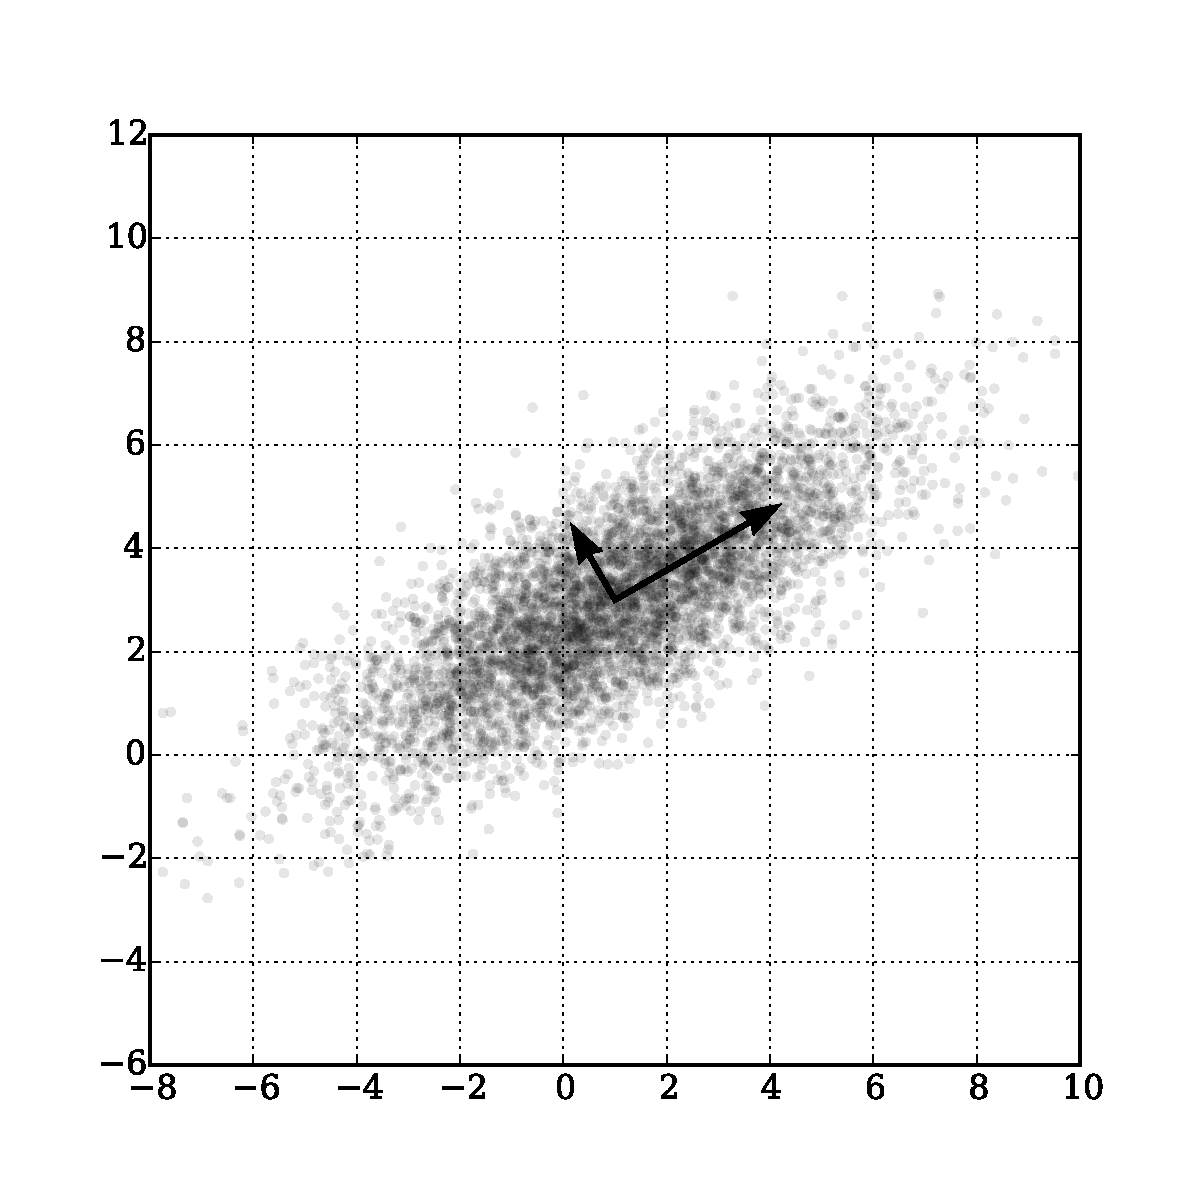
\includegraphics[width=\paperwidth,height=.6\paperheight,keepaspectratio]{../../pictures/pca}}

\tiny{\url{https://upload.wikimedia.org/wikipedia/commons/f/f5/GaussianScatterPCA.svg}}
\end{frame}



\begin{frame}[fragile,plain]{Preparation: Import modules and get some texts}
\begin{lstlisting}
from sklearn import datasets
from sklearn.decomposition import PCA
from sklearn.decomposition import TruncatedSVD
from sklearn.feature_extraction.text import CountVectorizer
from sklearn.pipeline import make_pipeline
from sklearn.preprocessing import FunctionTransformer
import matplotlib.pyplot as plt
%matplotlib inline

autotexts = datasets.fetch_20newsgroups('rec.autos', remove=('headers', 'footers', 'quotes'), subset='train')['data']
religiontexts = datasets.fetch_20newsgroups('soc.religion.christian', remove=('headers', 'footers', 'quotes'), subset='train')['data']

texts = autotexts[:20] + religiontexts[:20]
\end{lstlisting}
\end{frame}




\begin{frame}[fragile,plain]{Running PCA}
PCA does not accept a \textit{sparse matrix} as input (but the CountVectorizer gives one as output), so we need to transform it into a \textit{dense matrix}.

\begin{lstlisting}
myvec = CountVectorizer(texts, max_df=.5, min_df=5)
mypca = PCA(n_components=2)

mypipe = make_pipeline(myvec, FunctionTransformer(lambda x: x.todense(), accept_sparse=True), mypca)

r = mypipe.fit_transform(texts)
\end{lstlisting}
\end{frame}



%\begin{frame}[fragile,plain]{Plotting the result}
%\begin{lstlisting}
%plt.scatter([e[0] for e in r], [e[1] for e in r], alpha=.6)
%\end{lstlisting}

%\makebox[\linewidth]{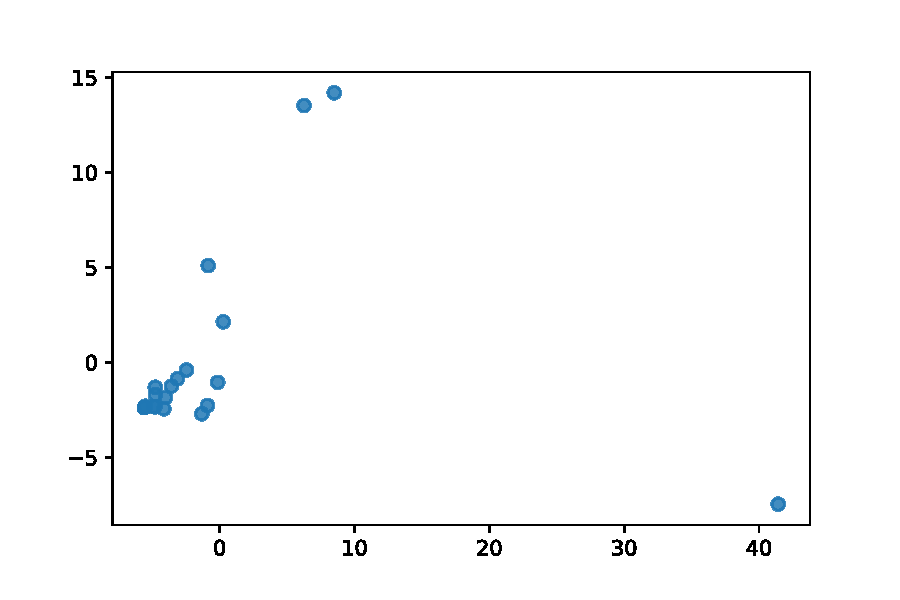
\includegraphics[width=\paperwidth,height=.6\paperheight,keepaspectratio]{../pictures/pca-example}}


%\end{frame}



\begin{frame}[fragile]{Singular value decomposition}
The need to use a dense matrix is \emph{really} a problem for large feature sets (which we have in NLP).
\pause

We therefore can better use SVD, which is essentially* the same and very simple to use:

\begin{lstlisting}
mysvd = TruncatedSVD(n_components=2)
mypipe = make_pipeline(myvec, mysvd)
r = mypipe.fit_transform(texts)
\end{lstlisting}

\footnotesize{(In this specific case, we even get exactly the same plot\ldots)}


\footnotesize{
* It's mathematically different, but SVD is even used ``under the hood'' by several PCA modules to solve PCA problems.

More info and background: \url{https://towardsdatascience.com/pca-and-svd-explained-with-numpy-5d13b0d2a4d8}}

\end{frame}


%\subsection{Multidimensional scaling}
%
%\begin{frame}[plain]
%\textbf{Finding similar variables}
%
%Multidimensional Scaling (MDS)
%\end{frame}
%
%\begin{frame}{Multidimensional scaling}
%Assume we have a $n \times n$ matrix in which in which the cell entries indicate the distance between ech of our $n$ features to each other feature based on their co-occurrence (= a dissimilarity matrix).
%\pause 
%
%MDS helps us visualising this in a two- or threedimensional space.
%
%\makebox[\linewidth]{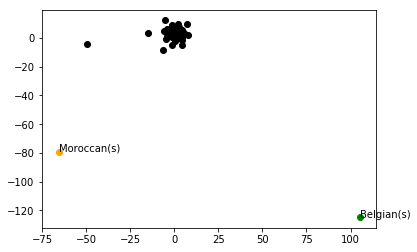
\includegraphics[width=\paperwidth,height=.5\paperheight,keepaspectratio]{../pictures/mds1}}
%\end{frame}
%
%
%\begin{frame}{Multidimensiponal scaling}
%\begin{itemize}
%\item Low-dimensional representation of the data in which the \textit{distances} respect well the distances in the original high-dimensional space
%\item With $D=2$ and $D=3$ often used for visualization (e.g., in political science)
%\end{itemize}
%\end{frame}









\section{Finding similar cases}

\subsection{k-means clustering}

\begin{frame}[plain]
\textbf{Finding similar cases}

k-means clustering
\end{frame}




\begin{frame}{Grouping features vs grouping cases}
Let's consider a corpus of several thousand user comments.

We could use SVD, MDS, or similar techniques to 
\begin{itemize}
\item figure out relationships between features
\item see which features stand out
\item get a first sense what topics are in the corpus.
\end{itemize}
\pause

But:
\begin{itemize}
\item<+-> We do not learn anything about \emph{which} texts (cases) belong to which topic
\item<+-> We could use the component scores returned by \texttt{.fit\_transform()} to then group our cases
\end{itemize}

\pause 
$\Rightarrow$ \footnotesize{Alternative: Choose the opposite approach and first find out which cases are most similar, \textit{then} describe what features characterize each group of cases}


\end{frame}




\begin{frame}{k-means clustering}
\begin{itemize}[<+->]
\item Goal: group cases into $k$ clusters
\item $k$ is set in advance
\item Algorithm to determine \textit{k} centroids (points in the middle of the cases that belong to it) such that the distances between the cases and their centroids are minimized
\item non-deterministic: starts with a randomly choosen centroids (there are other versions)
\item Cheap to compute: works even with large number of cases
\item We can run PCA first to reduce the number of features if we want/need to
\end{itemize}
\end{frame}




\begin{frame}{k-means clustering}
\makebox[\linewidth]{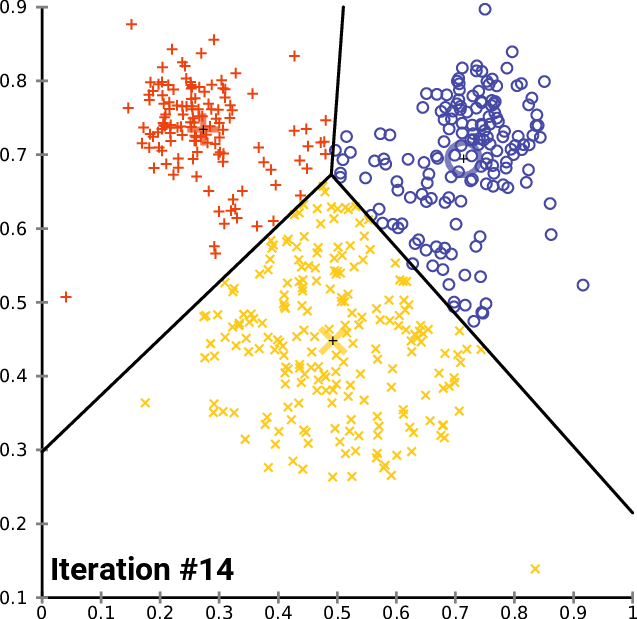
\includegraphics[width=\paperwidth,height=.65\paperheight,keepaspectratio]{../../pictures/kmeans}}

{\tiny{\url{https://upload.wikimedia.org/wikipedia/commons/e/ea/K-means\_convergence.gif}}}

Notice the big symbols indicating the centroids.
\end{frame}


\begin{frame}[plain,fragile]
\begin{lstlisting}
from sklearn.feature_extraction.text import TfidfVectorizer
from sklearn.cluster import KMeans

k = 5
texts = ['text1 ejkh ek ekh', 'ekyerykel'] # a list of texts

vec = TfidfVectorizer(min_df=5, max_df=.4)
features = vec.fit_transform(texts)
km = KMeans(n_clusters=k, init='k-means++', max_iter=100, n_init=1)
predictions = km.fit_predict(features)

\end{lstlisting}

That's it!
\pause

\begin{itemize}
\item \texttt{predictions} is a list of integers indicated the predicted cluster number. We can thus use \texttt{zip(predictions, texts)} to put them together.
\item<+-> We could also use \texttt{.fit()} and \texttt{.transform()} sperately and use our \texttt{km} to predict clusters for additional cases we have not used to train the model
\end{itemize}

\end{frame}


\begin{frame}[fragile,plain]{Let's get the terms closest to the centroids}
\begin{lstlisting}
order_centroids = km.cluster_centers_.argsort()[:, ::-1]
terms = vec.get_feature_names()

print("Top terms per cluster:")

for i in range(k):
    print("Cluster {}: ".format(i), end='')
for ind in order_centroids[i, :10]:
    print("{} ".format(terms[ind]), end='')
    print()
\end{lstlisting}
\pause
returns something like:

\begin{lstlisting}
Top terms per cluster:
Cluster 0: heard could if opinions info day how really just around 
Cluster 1: systems would ken pc am if as care summary ibm 
Cluster 2: year car years was my no one higher single than 
Cluster 3: which like seen 1000 few easily based personal work used 
Cluster 4: as was he if they my all will get has 
\end{lstlisting}
\end{frame}


\begin{frame}{Using k-means clustering\ldots}
\begin{itemize}
\item we get the cluster membership for each text; and
\item we get the terms that are most characteristic for the documents in each cluster.
\end{itemize}
\end{frame}

\begin{frame}{Finding the optimal $k$}

\begin{itemize}
\item The only way to find $k$ is to estimate multiple models with different $k$s
\item No single best solution; finding a balance between error within clusters (distances from centroid) and low number of clusters.
\item An elbow plot can be helpful (see example in Burscher et al, 2016)
\end{itemize}

\pause

\footnotesize 
Code-example for creating an elbow plot:
\url{https://pythonprogramminglanguage.com/kmeans-elbow-method/}

(Don't forget to insert \texttt{\%matplotlib inline} to actually see the plot)


\tiny{Burscher, B., Vliegenthart, R., \& de Vreese, C. H. (2016). Frames beyond words: Applying cluster and sentiment analysis to news coverage of the
nuclear power issue.\textit{ Social Science Computer Review, 34}(5), 530-545. doi:10.1177/0894439315596385}
\end{frame}


\subsection{Hierarchical clustering}

\begin{frame}[plain]
\textbf{Finding similar cases}

Hierarchical clustering
\end{frame}

\begin{frame}{Downsides of k-means clustering}
k-means is fast, but has problems:

\begin{itemize}
\item $k$ can only be determined by fitting multiple models and comparing them
\item bad results if the wrong $k$ is chosen
\item bad results if the (real) clusters are non-spherical
\item bad results if the (real) clusters are not evenly sized
\end{itemize}
\end{frame}


\begin{frame}{Hiearchical clusttering}
\begin{block}{General idea}
\begin{itemize}
\item To start, each case has its own cluster
\item Merge the two clusters that are most similar
\item Repeat until desired number of clusters is reached
\end{itemize}

\end{block}

\pause

\begin{block}{Different options}
\begin{itemize}
\item Stopping criterion: based on numerical statistic (e.g., Duda-Hart) or dendrogram
\item Linkage: how to determine which two clusters should be merged?
\end{itemize}

\end{block}
\end{frame}


\begin{frame}{Let's look into some options}

\url{https://scikit-learn.org/stable/modules/clustering.html\#hierarchical-clustering}

$\Rightarrow$ Ward's linkage is a good default all-rounder choice, especially if you encounter the problem that other linkages lead to almost all cases ending up in one cluster. 
\end{frame}


\begin{frame}{Hierarchical clustering takeaway}
\begin{itemize}
\item The main reason \emph{not} to use hierarchical methods (but k-means) is their computational cost: when clustering survey data of media users, never use $k$-means!
\item But for NLP/ML, costs may be too high (if not used carefully)
\item Very much worth considering, though, if you are really into grouping cases!
\end{itemize}
\end{frame}


\section{Important notes}
\begin{frame}[plain]
\textbf{Important notes for all types of clustering}
\end{frame}


\begin{frame}{Important notes}
\begin{block}{Consider the scales of measurement}
Clustering is based on distances -- if your features are not measured on the same scale, or if it is not meaningful to calculate a numerical distance, it won't produce meaningful results!

Consider standardizing/whitening your features!
\end{block}

\pause

\begin{block}{Pay attention outliers/extreme cases}
Extreme cases or outliers can have a strong influence.
\end{block}

\pause 
\begin{block}{Do proper pre-processing}
To reduce the number of features, but also to have \emph{meaningful} features (dimensions on which you expect high distances between the clusters).
\end{block}


\end{frame}



\begin{frame}[fragile,plain]{Exercise }
1. Go to \url{https://figshare.com/articles/News-Processed-Dataset/5296357} and download \texttt{WSJ\_20170607\_to\_20170726\_10AmTo4Pm.json} (the small file of 9 MB)


2. You can read the file as follows:\footnote{It's a json-lines file with one json object per line (see slides yesterday), and we only need what's withinthe \texttt{['content']} key, the rest is some metadata -- try out what happens if you leave away the \texttt{['content']}}

\begin{lstlisting}
import json
with open('WSJ_20170607_to_20170726_10AmTo4Pm.json') as f:
        texts = [json.loads(line)['content'] for line in f]
\end{lstlisting}




3. Use unsupervised machine learning techniques (and/or other techniques) to draw inferences about topics of (groups of) texts!
\end{frame}


\begin{frame}[plain]
This afternoon we will discuss one of the most popular unsupervised methods of the moment -- topic modeling.
\end{frame}


%\section[Recap]{Recap: PCA and Clustering}
%\begin{frame}{}
%Recap: PCA and Clustering
%\end{frame}
%\subsection*{PCA and Clustering}
%
%
%\begin{frame}{Let's assume we want to find out the topics in a large corpus of documents}
%We could either
%\begin{itemize}
%\item use PCA to find out related features (and interpret those as topics)
%\item or use clustering to find similar documents (and then look at the words they share to interpret as topics)
%\end{itemize}
%
%\pause
%
%Actually, we have \emph{two} things we want to model:
%
%\begin{enumerate}
%\item Which topics can we extract from the corpus?
%\item How present is each of these topics in each text in the corpus?
%\end{enumerate}
%
%\end{frame}


%\begin{frame}[fragile]{Recap: PCA}
%Document-term matrix
%\begin{lstlisting}
%w1,w2,w3,w4,w5,w6 ...
%text1, 2, 0, 0, 1, 2, 3 ...
%text2, 0, 0, 1, 2, 3, 4 ...
%text3, 9, 0, 1, 1, 0, 0 ...
%...
%\end{lstlisting}
%{\small{These can be simple counts, but also more advanced metrics, like tf-idf scores (where you weigh the frequency by the number of documents in which it occurs), cosine distances, etc.}}
%\pause
%\begin{itemize}
%\item given a term-document matrix, easy to do with any tool
%\item probably extremely skewed distributions
%\item some problematic assumptions: \textcolor{red}{does the goal of PCA, to find a solution in which one word loads on \emph{one} component match real life, where a word can belong to several topics or frames?}
%\end{itemize}
%
%\end{frame}


%\begin{frame}{Recap: clustering}
%\begin{itemize}
%\item given a term-document matrix, we can easily find clusters of documents that resemble each other
%\item but also here \textcolor{red}{does the goal of cluster analysis, assigning each document to \emph{one} cluster, match real life?}
%\end{itemize}
%\end{frame}
%
%
%\begin{frame}{We need other models to}
%\begin{enumerate}[<+->]
%\item model \emph{simultaneously} (a) which topics we find in the whole corpus, and (b) which of these topics are present in which document; while at the same time
%\item allowing (a) words to be part of multiple topics, and (b) multiple topics to be present in one document; and
%\item being able to make connections between words ``even if they never actually occured in a document together'' (Maier et al, 2018, p.~96)
%\end{enumerate}
%
%\tiny{Maier, D., Waldherr, A., Miltner, P., Wiedemann, G., Niekler, A., Keinert, A., \ldots Adam, S. (2018). Applying LDA Topic Modeling in Communication Research: Toward a Valid and Reliable Methodology. \textit{Communication Methods and Measures, 12}(2--3), 93--118. doi:10.1080/19312458.2018.1430754}
%\end{frame}



%\section{LDA Topic models}
%
%\subsection{An introduction to LDA}
%
%\begin{frame}{}
%Enter \textbf{topic modeling with Latent Dirichlet Allocation (LDA)}
%\end{frame}
%
%
%
%
%
%
%\begin{frame}{LDA, what's that?}
%\begin{block}{No mathematical details here, but the general idea}
%\begin{itemize}
%\item There are $k$ topics, $T_1$\ldots$T_k$
%\item Each document $D_i$ consists of a mixture of these topics, e.g.$80\% T_1, 15\% T_2, 0\% T_3, \ldots 5\% T_k $
%\item On the next level, each topic consists of a specific probability distribution of words
%\item Thus, based on the frequencies of words in $D_i$, one can infer its distribution of topics
%\item Note that LDA (like PCA) is a Bag-of-Words (BOW) approach
%\end{itemize}
%\end{block}
%
%\end{frame}
%
%
%
%
%\begin{frame}[fragile]{Doing a LDA in Python}
%You can use gensim ({\v R}eh{\r u}{\v r}ek \& Sojka, 2010) for this.
%
%Let us assume you have a list of lists of words (!) called \texttt{texts}:
%
%\begin{lstlisting}
%articles=['The tax deficit is higher than expected. This said xxx ...', 'Germany won the World Cup. After a']
%texts=[art.split() for art in articles]
%\end{lstlisting}
%which looks like this:
%\begin{lstlisting}
%[['The', 'tax', 'deficit', 'is', 'higher', 'than', 'expected.', 'This', 'said', 'xxx', '...'], ['Germany', 'won', 'the', 'World', 'Cup.', 'After', 'a']]
%\end{lstlisting}
%
%\tiny{{\v R}eh{\r u}{\v r}ek, R., \& Sojka, P. (2010). Software framework for topic modelling with large corpora. \emph{Proceedings of the LREC 2010 Workshop on New Challenges for NLP Frameworks}, pp. 45–50. Valletta, Malta: ELRA. }
%
%\end{frame}
%
%
%
%
%\begin{frame}[plain,fragile]
%\begin{lstlisting}
%from gensim import corpora, models
%
%NTOPICS = 100
%LDAOUTPUTFILE="topicscores.tsv"
%
%# Create a BOW represenation of the texts
%id2word = corpora.Dictionary(texts)
%mm =[id2word.doc2bow(text) for text in texts]
%
%# Train the LDA models.
%mylda = models.ldamodel.LdaModel(corpus=mm, id2word=id2word, num_topics=NTOPICS, alpha="auto")
%
%# Print the topics.
%for top in mylda.print_topics(num_topics=NTOPICS, num_words=5):
%print ("\n",top)
%
%print ("\nFor further analysis, a dataset with the topic score for each document is saved to",LDAOUTPUTFILE)
%
%scoresperdoc=mylda.inference(mm)
%
%with open(LDAOUTPUTFILE,"w",encoding="utf-8") as fo:
%for row in scoresperdoc[0]:
%fo.write("\t".join(["{:0.3f}".format(score) for score in row]))
%fo.write("\n")
%\end{lstlisting}
%
%\end{frame}
%
%
%\begin{frame}[fragile]{Output: Topics (below) \& topic scores (next slide)}
%\begin{lstlisting}
%0.069*fusie + 0.058*brussel + 0.045*europesecommissie + 0.036*europese + 0.023*overname
%0.109*bank + 0.066*britse + 0.041*regering + 0.035*financien + 0.033*minister
%0.114*nederlandse + 0.106*nederland + 0.070*bedrijven + 0.042*rusland + 0.038*russische
%0.093*nederlandsespoorwegen + 0.074*den + 0.036*jaar + 0.029*onderzoek + 0.027*raad
%0.099*banen + 0.045*jaar + 0.045*productie + 0.036*ton + 0.029*aantal
%0.041*grote + 0.038*bedrijven + 0.027*ondernemers + 0.023*goed + 0.015*jaar
%0.108*werknemers + 0.037*jongeren + 0.035*werkgevers + 0.029*jaar + 0.025*werk
%0.171*bank + 0.122* + 0.041*klanten + 0.035*verzekeraar + 0.028*euro
%0.162*banken + 0.055*bank + 0.039*centrale + 0.027*leningen + 0.024*financiele
%0.052*post + 0.042*media + 0.038*nieuwe + 0.034*netwerk + 0.025*personeel
%...
%\end{lstlisting}
%\end{frame}
%
%
%\begin{frame}[plain]
%\makebox[\linewidth]{
%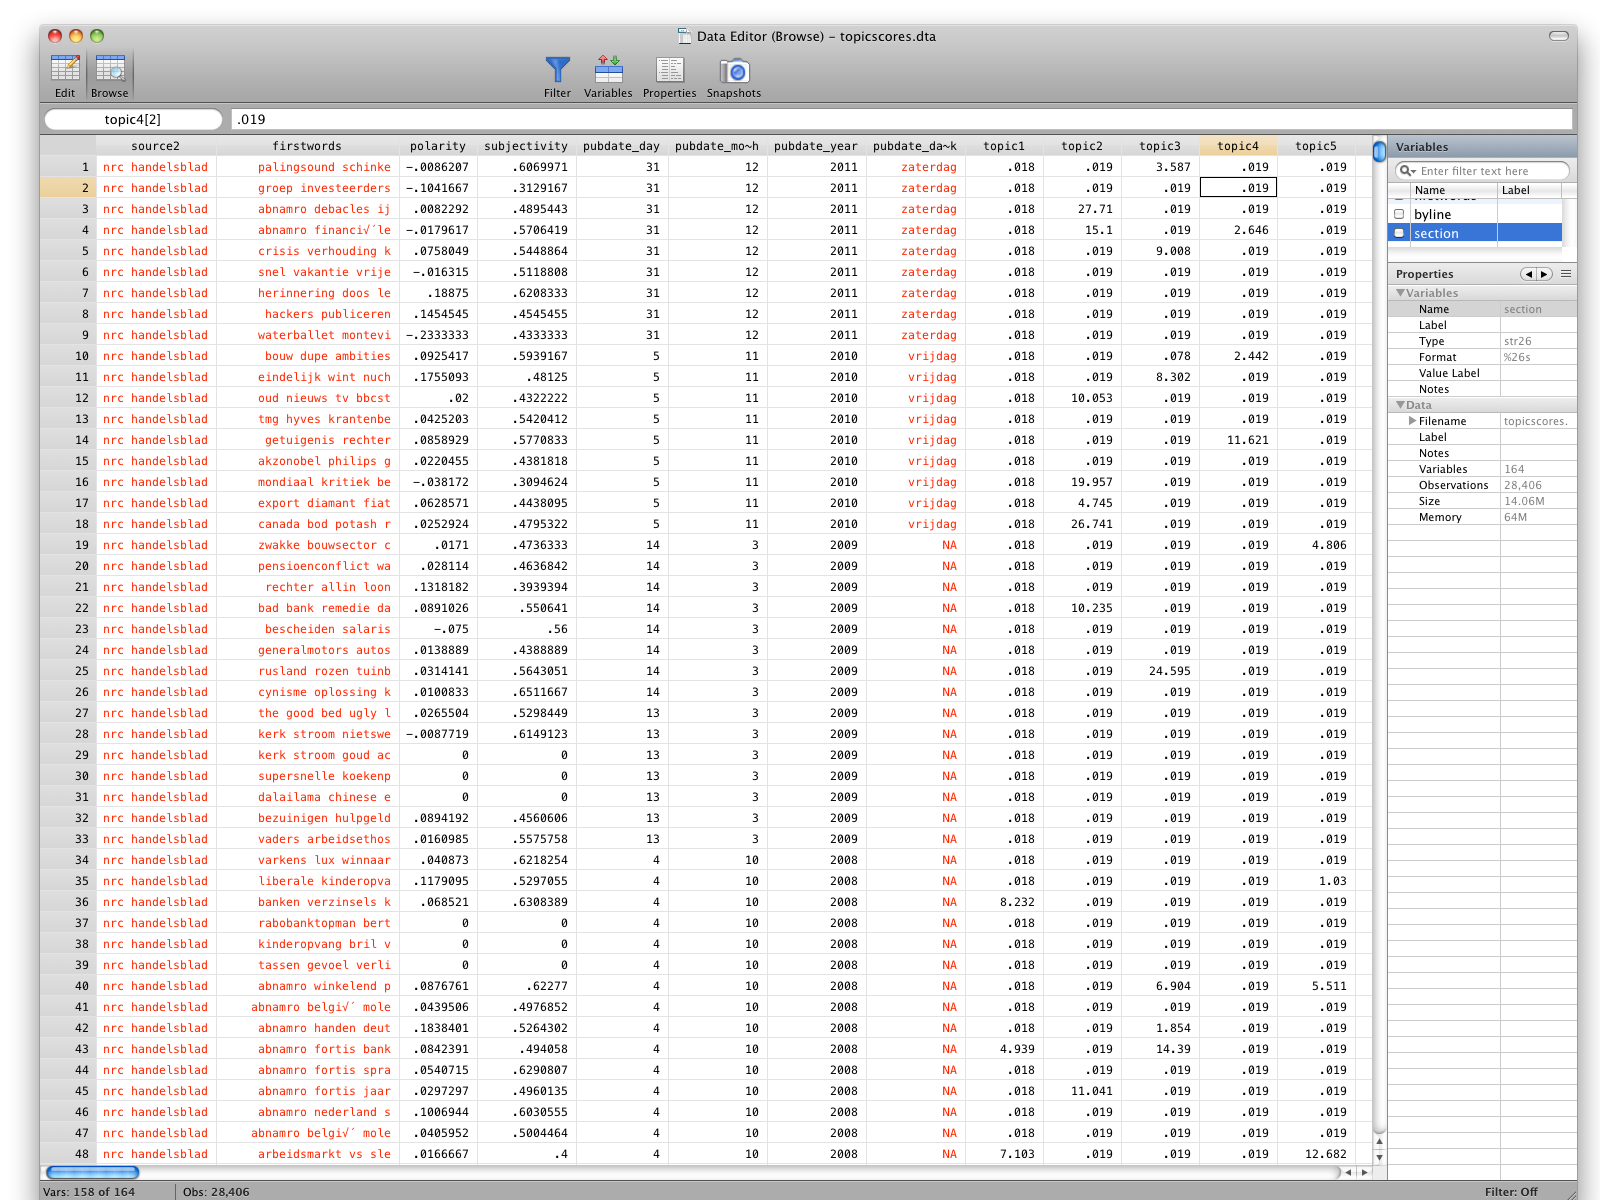
\includegraphics[width=\paperwidth,height=\paperheight,keepaspectratio]{../pictures/topicscores}}
%\end{frame}
%
%
%
%
%\begin{frame}[fragile]{Visualization with pyldavis}
%\begin{lstlisting}
%import pyLDAvis
%import pyLDAvis.gensim
%# first estiate gensim model, then:
%vis_data = pyLDAvis.gensim.prepare(mylda,mm,id2word)
%pyLDAvis.display(vis_data)
%\end{lstlisting}
%\makebox[\linewidth]{
%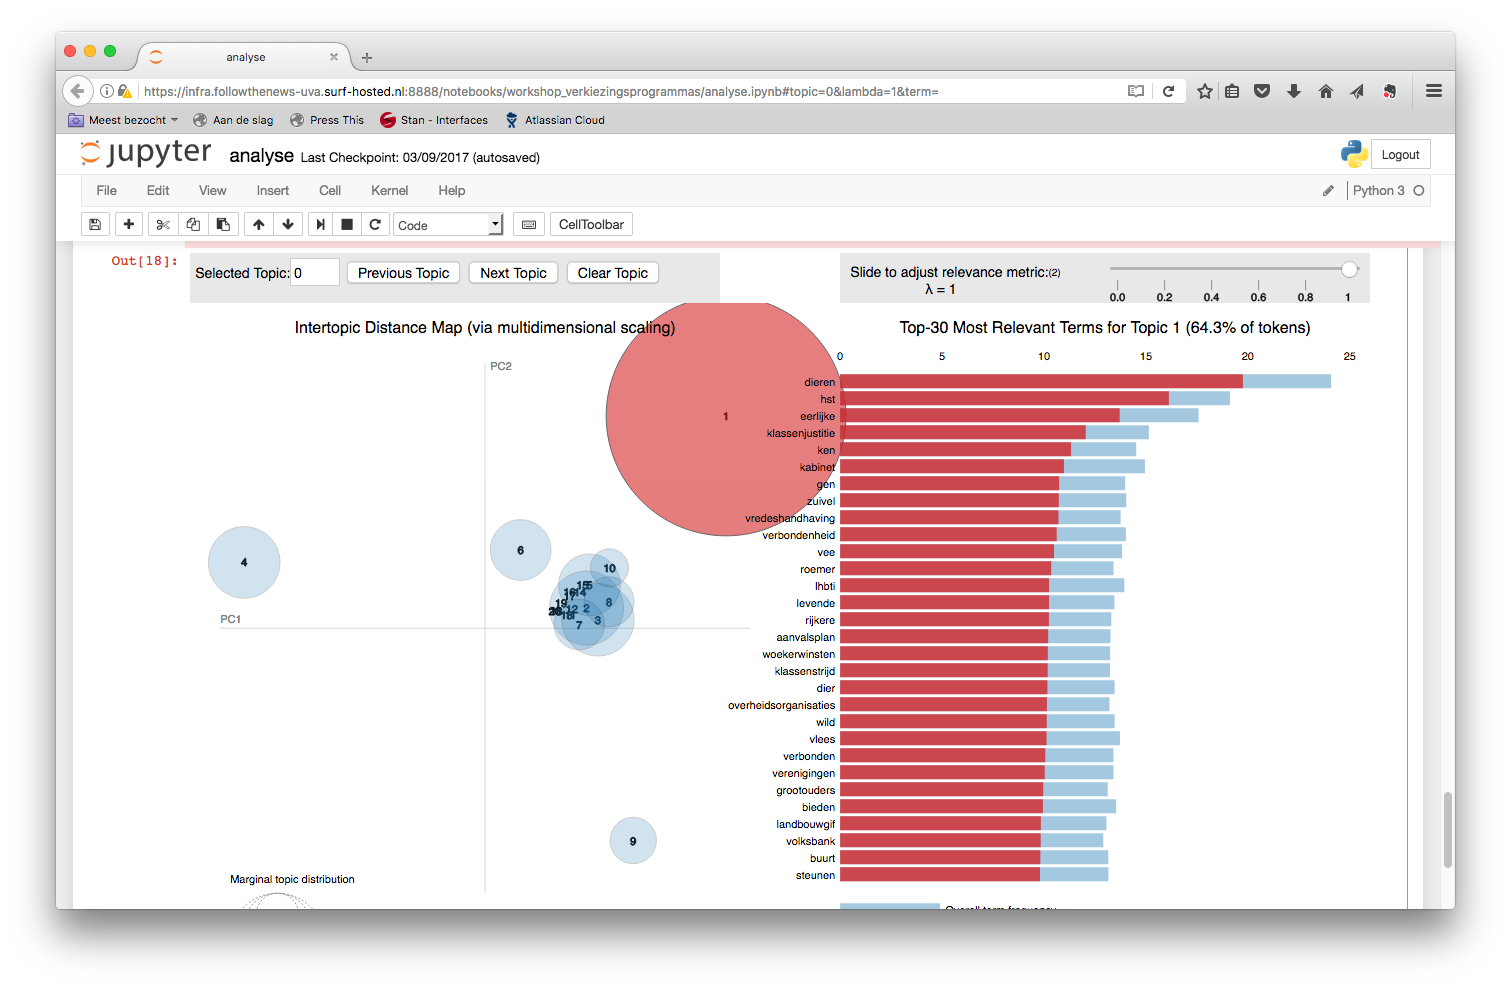
\includegraphics[width=\paperwidth,height=.5\paperheight,keepaspectratio]{../pictures/pyldavis}}
%\end{frame}
%
%\begin{frame}{Visualization with pyldavis}
%Short note about the $\lambda$ setting:
%
%It influences the ordering of the words in pyldavis.
%
%\begin{quote}
%``For $\lambda = 1$, the ordering of the top words is equal to the ordering of the standard conditional word probabilities. For $\lambda$ close to zero, the most specific words of the topic will lead the list of top words. In their case study, Sievert and Shirley (2014, p. 67) found the best interpretability of topics using a  $\lambda$-value close to .6, which we adopted for our own case'' (Maier et al., 2018, p.~107)
%\end{quote}
%
%
%\tiny{Maier, D., Waldherr, A., Miltner, P., Wiedemann, G., Niekler, A., Keinert, A., \ldots Adam, S. (2018). Applying LDA Topic Modeling in Communication Research: Toward a Valid and Reliable Methodology. \textit{Communication Methods and Measures, 12}(2--3), 93--118. doi:10.1080/19312458.2018.1430754}
%\end{frame}
%
%\begin{frame}[plain]{Code examples}
%
%
%\url{https://github.com/damian0604/bdaca/blob/master/rm-course-2/week12/lda.ipynb}
%\end{frame}
%
%
%
%\subsection{Choosing the best (or a good) topic model}
%
%\begin{frame}{Choosing the best (or a good) topic model}
%\begin{itemize}
%\item There is no single best solution (e.g., do you want more coarse of fine-grained topics?)
%\item Non-deterministic
%\item Very sensitive to preprocessing choices
%\item Interplay of both metrics and (qualitative) interpretability 
%\end{itemize}
%
%See for more elaborate guidance:
%
%\tiny{Maier, D., Waldherr, A., Miltner, P., Wiedemann, G., Niekler, A., Keinert, A., \ldots Adam, S. (2018). Applying LDA Topic Modeling in Communication Research: Toward a Valid and Reliable Methodology. \textit{Communication Methods and Measures, 12}(2--3), 93--118. doi:10.1080/19312458.2018.1430754}
%
%\end{frame}
%
%
%
%\begin{frame}{Evaluation metrics (closer to zero is better)}
%\begin{block}{perplexity}
%A goodness-of-fit measure, answering the question: If we do a train-test split, how well does the trained model fit the test data?
%\end{block}
%
%\pause 
%\begin{block}{coherence}
%\begin{itemize}
%\item mean coherence of the whole model: attempts to quantify the interpretability
%\item coherence per topic: allows to get topics that are most likely to be coherently interpreted (\texttt{.top\_topics()})
%\end{itemize}
%\end{block}
%
%\end{frame}
%
%
%\begin{frame}{So, how do we do this?}
%\begin{itemize}[<+->]
%\item Basically, similar to the idea behind our grid search from two weeks ago: estimate multiple models, store the metrics for each model, and then compare them (numerically, or by plotting)
%\item Idea: We select some candidate models, and then look whether they can be interpreted.
%\item But what can we tune?
%\end{itemize}
%\end{frame}
%
%
%\begin{frame}{Choosing $k$: How many topics do we want?}
%\begin{itemize}
%\item Typical values: $10<k<200$
%\item Too low: losing nuance, so broad it becomes meaningless
%\item Too high: picks up tiny pecularities instead of finding general patterns
%\item There is no inherent ordering of topics (unlike PCA!)
%\item We can throw away or merge topics later, so if out of $k=50$ topics 5 are not interpretable and a couple of others overlap, it still may be a good model
%\end{itemize}
%\end{frame}
%
%
%\begin{frame}[fragile]{Choosing $\alpha$: how sparse should the document-topic distribution $\theta$ be?}
%\begin{itemize}
%\item The higher $\alpha$, the more topics per document 
%\item Default: $1/k$
%\item But: We can explicitly change it, or -- really cool -- even learn $\alpha$ from the data (\texttt{alpha = "auto"})
%\end{itemize}
%
%\pause 
%
%Takeaway: It takes longer, but you probably want to learn alpha from the data, using multiple passes:
%
%\begin{lstlisting}
%mylda LdaModel(corpus=tfidfcorpus[ldacorpus], id2word=id2word, num_topics=50, alpha='auto', passes=10)
%\end{lstlisting}
%
%
%\end{frame}
%
%
%\begin{frame}{Choosing $\eta$: how sparse should the topic-word distribution $\lambda$ be?}
%\begin{itemize}
%\item Can be used to boost specific words
%\item Can also be learned from the data 
%\end{itemize}
%
%\pause
%Takeaway: Even though you can do \texttt{eta="auto"}, this usually does not help you much.
%
%\end{frame}
%
%
%% \subsection{Drawbacks of LDA topic models}
%
%
%\subsection{Using topic models}
%
%\begin{frame}{Using topic models}
%
%You got your model -- what now?
%
%\begin{enumerate}
%\item Assign topic scores to documents
%\item Label topics
%\item Merge topics, throw away boilerplate topics and similar (manually, or aided by cluster analysis)
%\item Compare topics between, e.g., outlets
%\item or do some time-series analysis.
%\end{enumerate}
%
%
%Example:
%\tiny{Tsur, O., Calacci, D., \& Lazer, D. (2015). A Frame of Mind: Using Statistical Models for Detection of Framing and Agenda Setting Campaigns. \textit{Proceedings of the 53rd Annual Meeting of the Association for Computational Linguistics and the 7th International Joint Conference on Natural Language Processing} (pp. 1629–1638).}
%
%
%
%\end{frame}
%
%
%
%\subsection{Other forms of topic models}
%
%
%\begin{frame}[plain]
%Other forms of topic models
%\end{frame}
%
%\begin{frame}{Other forms of topic models}
%\begin{itemize}
%\item Author-topic models
%\item Structural topic models
%\item Non-negative matrix factorization
%\item \ldots
%\end{itemize}
%\end{frame}




\end{document}
